% Notes
% ========== Introduction
% - Ordinateur quantiques, n'existent pas encore ==> Rajouter une slide sur les ordinateurs quantiques
% - Parler de Bob = serveur
% - Qubits servent à cacher les calculs. Alice doit avoir un petit ordinateur quantique

% TODO : mettre la photo du qubit à l'étape précédente
% TODO : Animation avec le plus qui s'ouvre
% TODO : boite noire ?

\documentclass[]{beamer}

% \includeonlyframes{currentf}
% \usepackage[T1]{fontenc}
\usepackage[utf8]{inputenc}
\usepackage[english]{babel}     
\usepackage{siunitx}
\usepackage{etoolbox}
\usepackage{listings}
\usepackage{color}
% ffmpeg -framerate 24 -i %04d.png qubit_projection.mp4
% ffmpeg -framerate 24 -start_number 94 -i %04d.png qubit_projection.mp4 
% \usepackage[]{qcircuit}


\usefonttheme[onlymath]{serif}

\newcommand*{\cB}{\mathcal{B}}
\newcommand*{\cC}{\mathcal{C}}
\newcommand*{\cD}{\mathcal{D}}
\newcommand*{\cE}{\mathcal{E}}
\newcommand*{\cF}{\mathcal{F}}
\newcommand*{\cG}{\mathcal{G}}
\newcommand*{\cH}{\mathcal{H}}
\newcommand*{\cI}{\mathcal{I}}
\newcommand*{\cM}{\mathcal{M}}
\newcommand*{\cN}{\mathcal{N}}
\newcommand*{\cP}{\mathcal{P}}
\newcommand*{\cQ}{\mathcal{Q}}
\newcommand*{\cR}{\mathcal{R}}
\newcommand*{\cS}{\mathcal{S}}
\newcommand*{\cT}{\mathcal{T}}
\newcommand*{\cU}{\mathcal{U}}
\newcommand*{\cV}{\mathcal{V}}
\newcommand*{\cW}{\mathcal{W}}
\newcommand*{\cX}{\mathcal{X}}
\newcommand*{\cY}{\mathcal{Y}}
\newcommand*{\cZ}{\mathcal{Z}}

\newcommand*{\id}{\mathrm{id}}
\newcommand*{\tr}{\mathrm{tr}}
\newcommand{\ket}[1]{\ensuremath{|#1\rangle}}
\newcommand{\bra}[1]{\ensuremath{\langle #1|}}
% \newcommand*{\ket}[1]{| #1 \rangle}
% \newcommand*{\bra}[1]{\langle #1 |}
\newcommand*{\spr}[2]{\langle #1 | #2 \rangle}
\newcommand*{\proj}[1]{|#1\rangle\!\langle #1|}

\newcommand*\xor{\mathbin{\oplus}}

\newcommand*{\eps}[0]{\varepsilon}
\newcommand*{\D}[0]{\mathbb{D}}
\newcommand*{\C}[0]{\mathbb{C}}
\newcommand*{\N}[0]{\mathbb{N}}
\newcommand*{\R}[0]{\mathbb{R}}
\newcommand*{\Z}[0]{\mathbb{Z}}

\newcommand{\cqubit}[1]{\raisebox{-.5\height}{\includegraphics[width=0.9cm]{figures/qubit_#1.png}}}
\newcommand{\cotimes}{\raisebox{-.5\height}{$\otimes$}}

\usepackage{multimedia}

\usepackage{cancel} % Barer des équations
\newcommand<>{\xxcancel}[1]{\alt#2{\xcancel{#1}\vphantom{#1}}{#1}}

\usepackage{tikz}
\usetikzlibrary{shapes.geometric,arrows,arrows.meta,shadows}
\usetikzlibrary{mindmap,backgrounds,positioning}
\usetikzlibrary{automata,positioning,fit,backgrounds}
\usetikzlibrary{positioning,arrows,matrix,calc,math}
\usepgflibrary{decorations.pathreplacing}
\usetikzlibrary{decorations.pathmorphing}
\usetikzlibrary{shapes.callouts}


\tikzset{my snake/.style={decorate,decoration={snake,amplitude=.4mm,segment length=2mm,post length=2mm}}}

\pgfdeclarelayer{background}
\pgfdeclarelayer{foreground}
\pgfsetlayers{background,main,foreground}   %% some additional layers for demo


\usetheme{Warsaw}
% \graphicspath{{pictures/}} % on change la racine des images

\usepackage [
  n,
  advantage,
  operators,
  sets,
  adversary,
  landau,
  probability,
  notions,
  logic,
  ff,
  mm,
  primitives,
  events,
  complexity,
  asymptotics,
  keys
  ] {cryptocode}

\renewcommand{\sample}[0]{\xleftarrow{\text{\tiny \$}}}

\usepackage[skins,many]{tcolorbox}
\newtcolorbox{subproof}{
  breakable,
  enhanced,
  frame hidden,
  interior hidden,
  opacityback=0,
  colframe=black,
  sharp corners,
  top = 0px, before skip = 0.1cm,
  bottom = 0px, after  skip = 0.1cm,  
  left=0.1cm, left skip=0.1cm,
  right=0px, right skip=0px,
  borderline west={0.02cm}{0pt}{black}
}

\usepackage{MyMnSymbol}

\definecolor{mygreen}{rgb}{0,0.6,0}
\definecolor{mygray}{rgb}{0.5,0.5,0.5}
\definecolor{mymauve}{rgb}{0.58,0,0.82}

\lstset{ %
  backgroundcolor=\color{white},   % choose the background color; you must add \usepackage{color} or \usepackage{xcolor}
  basicstyle=\footnotesize,        % the size of the fonts that are used for the code
  breakatwhitespace=false,         % sets if automatic breaks should only happen at whitespace
  breaklines=true,                 % sets automatic line breaking
  captionpos=b,                    % sets the caption-position to bottom
  commentstyle=\color{mygreen},    % comment style
  deletekeywords={...},            % if you want to delete keywords from the given language
  escapeinside={\%*}{*)},          % if you want to add LaTeX within your code
  extendedchars=true,              % lets you use non-ASCII characters; for 8-bits encodings only, does not work with UTF-8
  frame=single,	                   % adds a frame around the code
  keepspaces=true,                 % keeps spaces in text, useful for keeping indentation of code (possibly needs columns=flexible)
  keywordstyle=\color{blue},       % keyword style
  language=Octave,                 % the language of the code
  otherkeywords={*,...},           % if you want to add more keywords to the set
  numbers=left,                    % where to put the line-numbers; possible values are (none, left, right)
  numbersep=5pt,                   % how far the line-numbers are from the code
  numberstyle=\tiny\color{mygray}, % the style that is used for the line-numbers
  rulecolor=\color{black},         % if not set, the frame-color may be changed on line-breaks within not-black text (e.g. comments (green here))
  showspaces=false,                % show spaces everywhere adding particular underscores; it overrides 'showstringspaces'
  showstringspaces=false,          % underline spaces within strings only
  showtabs=false,                  % show tabs within strings adding particular underscores
  stepnumber=2,                    % the step between two line-numbers. If it's 1, each line will be numbered
  stringstyle=\color{mymauve},     % string literal style
  tabsize=2,	                   % sets default tabsize to 2 spaces
  title=\lstname                   % show the filename of files included with \lstinputlisting; also try caption instead of title
}

\newcommand{\includepdfpages}[1]{%
  \pdfximage{#1}%
  \foreach \ov in {1,...,\the\pdflastximagepages}{%
    \includegraphics<+>[page=\ov]{#1}%
  }%
}

\newcommand{\includepdfpageswidth}[2]{%
  \pdfximage{#2}%
  \foreach \ov in {1,...,\the\pdflastximagepages}{%
    \includegraphics<+>[page=\ov,width=#1]{#2}%
  }%
}

\newcommand{\includetikzpdfpageswidth}[3]{%
  \pdfximage{#2}%
  \foreach \ov in {1,...,\the\pdflastximagepages}{%
    \onslide<+>{\node[#3]{\includegraphics[page=\ov,width=#1]{#2}};}%
  }%
}

\newcommand{\includetikzpdfpages}[2]{%
  \pdfximage{#1}%
  \foreach \ov in {1,...,\the\pdflastximagepages}{%
    \onslide<+>{\node[#2]{\includegraphics[page=\ov]{#1}};}%
  }%
}

\newcommand{\includetikzpdfpageskeeplast}[2]{%
  \pdfximage{#1}%
  \pgfmathparse{\the\pdflastximagepages-1}
  \foreach \ov in {1,...,\pgfmathresult}{%
    \onslide<+>{\node[#2]{\includegraphics[page=\ov]{#1}};}%
  }%
  \onslide<+->{\node[#2]{\includegraphics[page=\the\pdflastximagepages]{#1}};}%
}

\newcommand{\tcancel}[1]{\ensuremath{\xcancel{\text{#1}}}}

%%% Local Variables:
%%% mode: latex
%%% TeX-master: t
%%% End:


% \usepackage{thmtools}
% \let\definition\relax
% \declaretheorem[name=Definition]{definition}
% \declaretheorem[name=Theorem]{theorem}
% \declaretheorem[name=Lemma,sibling=theorem]{lemma}


\setbeamerfont{subsection in toc}{size=\small}
\AtBeginSection[]
{
  \begin{frame}<beamer>
    \frametitle{Plan}
    \tableofcontents[currentsection]
  \end{frame}
}

\defbeamertemplate*{footline}{shadow theme}{%
  \leavevmode%
  \hbox{\begin{beamercolorbox}[wd=.5\paperwidth,ht=2.5ex,dp=1.125ex,leftskip=.3cm plus1fil,rightskip=.3cm]{author in head/foot}%
      \usebeamerfont{author in head/foot}\hfill\insertshortauthor
    \end{beamercolorbox}%

    \begin{beamercolorbox}[wd=.5\paperwidth,ht=2.5ex,dp=1.125ex,leftskip=.3cm,rightskip=.3cm plus1fil]{title in head/foot}%
      \usebeamerfont{title in head/foot}\insertshorttitle\hfill%
      \insertframenumber\,/\,\inserttotalframenumber
    \end{beamercolorbox}}%
  \vskip0pt%
}

% Bigger margin
\newcommand\Wider[2][3em]{%
\makebox[\linewidth][c]{%
  \begin{minipage}{\dimexpr\textwidth+#1\relax}
  \raggedright#2
  \end{minipage}%
  }%
}

\title[Classically Driven Blind Quantum Computing]{On the possibility of classical client blind quantum computing}
\author{Alexandru Cojocaru, Léo Colisson, Elham Kashefi, Petros Wallden}
% \institute{École Normale Supérieure (ENS) Paris-Saclay, Département Informatique\\Laboratory for Foundations of Computer Science, University of Edinburgh,\\sous la direction d'Elham Kashefi}

\begin{document}
% ==================================================

\begin{frame}
  \titlepage
\end{frame}
% ==================================================

\begin{frame}
  \tableofcontents
\end{frame}

% ==================================================

\section{Motivations}

\subsection{Main Goal}

\begin{frame}{Main Goal}
  \begin{figure}[ht]
    \centering
    \begin{tikzpicture}
      % Alice
      \node[inner sep=0pt](alice)    {
\includegraphics[width=.20\textwidth]{figures/aliceteacup.png}};
      % Bob
      \node<1>[inner sep=0pt,right=.50\textwidth of alice](bob) {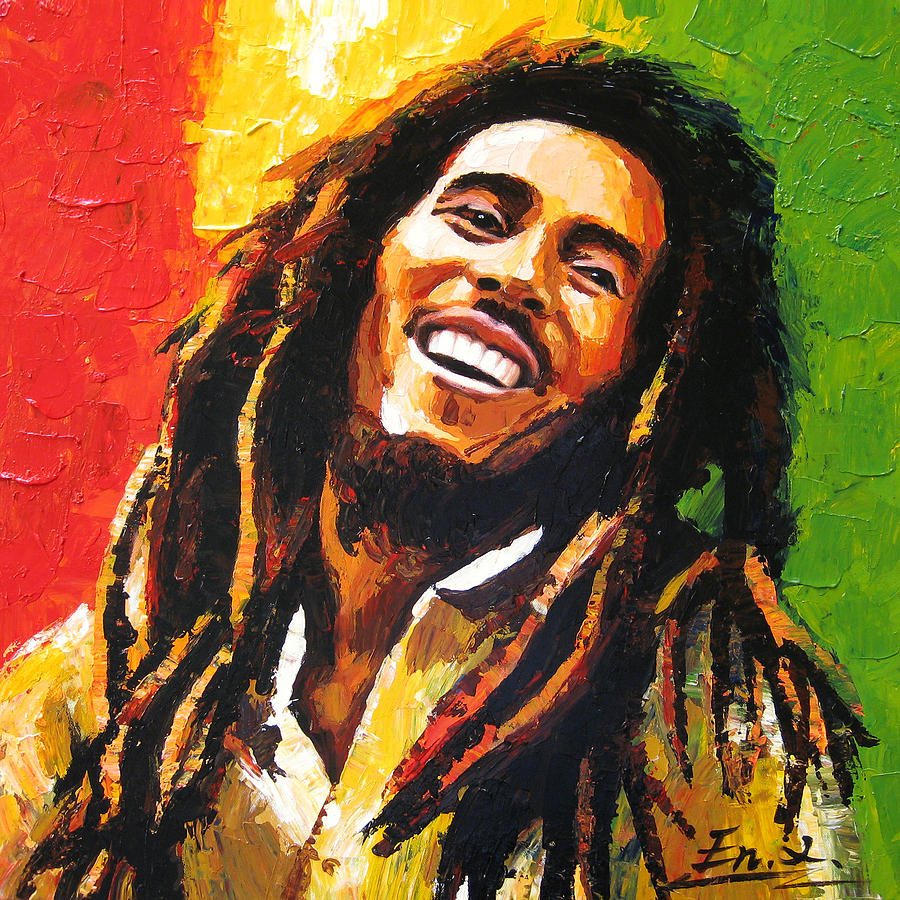
\includegraphics[width=.20\textwidth]{figures/bob_marley.jpg}};
      % Bob Marley aveugle
      \node<2->[inner sep=0pt,right=.50\textwidth of alice](bob) {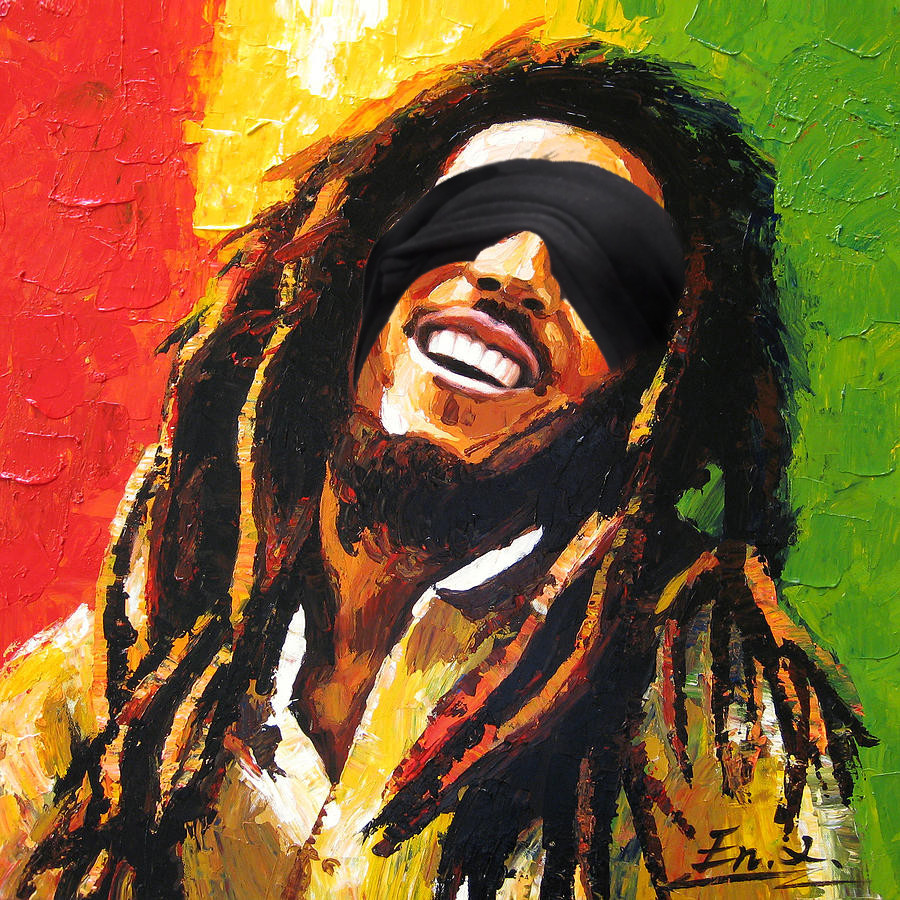
\includegraphics[width=.20\textwidth]{figures/bob_marley_aveugle.jpg}};
      % Petit ordinateur
      \node[inner sep=0pt,below=.04\textwidth of alice](petitordi) {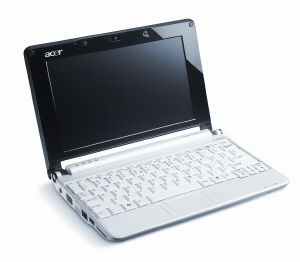
\includegraphics[width=.20\textwidth]{figures/petit_ordinateur.jpg}};
      % Ordinateur quantique
      \node[inner sep=0pt,below=.04\textwidth of bob](ordiquantique) {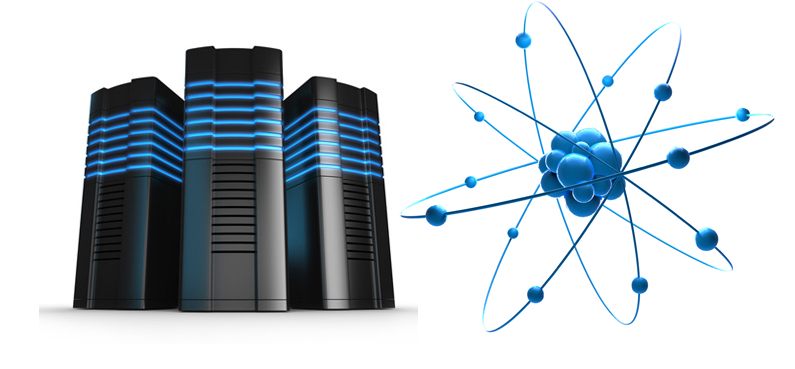
\includegraphics[width=.35\textwidth]{figures/ordi_quantique.png}};
      % Flèches
      \draw<1>[-latex] ([yshift=.04\textwidth]petitordi.east) -- ([yshift=.04\textwidth]ordiquantique.west |- petitordi.west);
      \draw[-latex] ([yshift=-.04\textwidth]ordiquantique.west |- petitordi.west) -- ([yshift=-.04\textwidth]petitordi.east);
      % Flèche logo atome
      \draw<2>[-latex] ([yshift=.04\textwidth]petitordi.east) -- ([yshift=.04\textwidth]ordiquantique.west |- petitordi.west) node[midway,above] {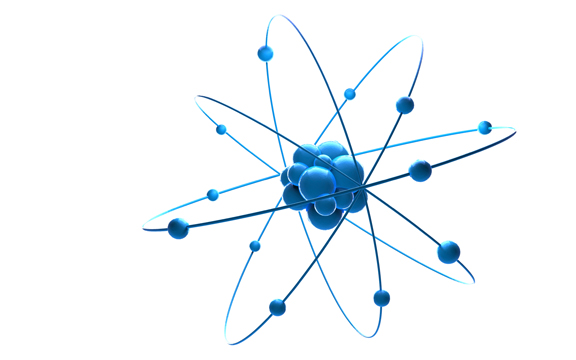
\includegraphics[width=.15\textwidth]{figures/atome.png}};
      % Flèche logo atome barré
      \draw<3>[-latex] ([yshift=.04\textwidth]petitordi.east) -- ([yshift=.04\textwidth]ordiquantique.west |- petitordi.west) node[midway,above](petit_atome_barre) {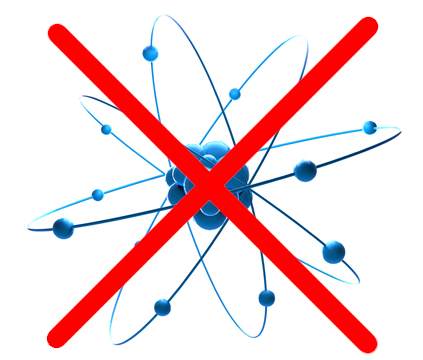
\includegraphics[width=.15\textwidth]{figures/atome_barre.png}};
      \node<3>[above=.02\textwidth of petit_atome_barre] {{\Large \textbf{\textcolor{red}{?}}}};
    \end{tikzpicture}
    \caption{(Blind) Quantum Computing}
  \end{figure}
\end{frame}

\subsection{Other Applications}

\begin{frame}{Other Applications}
  \begin{figure}[ht]
    \centering
    \scalebox{.7}{
      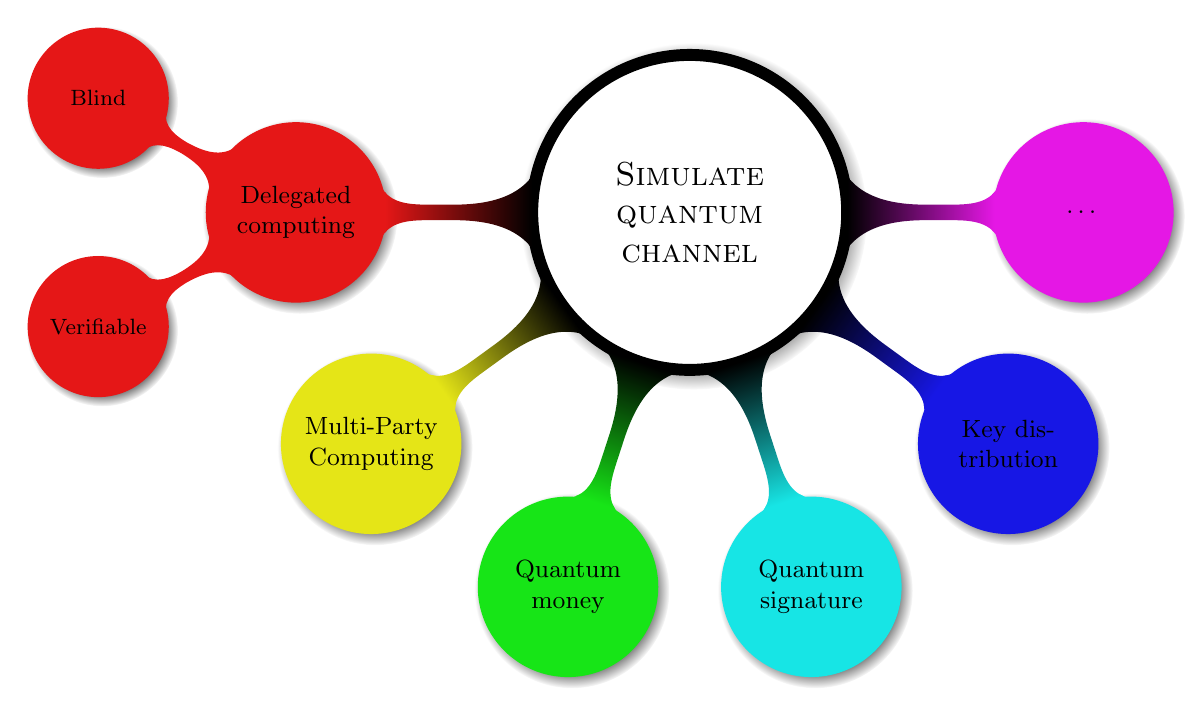
\begin{tikzpicture}[rotate=-90]
        \colorlet{color min hsb}[hsb]{red}
        \colorlet{color max hsb}[hsb]{magenta}
        \def\bl{90}
        \colorlet{colorA}[rgb]{color max hsb!0!color min hsb!\bl!black}
        \colorlet{colorB}[rgb]{color max hsb!20!color min hsb!\bl!black}
        \colorlet{colorC}[rgb]{color max hsb!40!color min hsb!\bl!black}
        \colorlet{colorD}[rgb]{color max hsb!60!color min hsb!\bl!black}
        \colorlet{colorE}[rgb]{color max hsb!80!color min hsb!\bl!black}
        \colorlet{colorF}[rgb]{color max hsb!100!color min hsb!\bl!black}
        
        \path[mindmap,
          every node/.style={concept, circular drop shadow,execute at begin node=\hskip0pt},
          concept color=black,text=black,font=\bfseries,
          grow cyclic,
          root concept/.append style={
            concept color=black, fill=white, line width=1ex, text=black,
            font=\large\scshape},
          level 1 concept/.append style={sibling angle=180/5}]
        
        node[concept, root concept] {Simulate quantum channel}
        child[concept color=colorA] {
          node[concept] {Delegated computing}
          child { node[concept] {Blind} }
          child { node[concept] {Verifiable} }
        }  
        child[concept color=colorB] {
          node[concept] {Multi-Party Computing}
        }
        child[concept color=colorC] {
          node[concept] {Quantum money}
        }
        child[concept color=colorD] {
          node[concept] {Quantum signature}
        }
        child[concept color=colorE] {
          node[concept] {Key distribution}
        }
        child[concept color=colorF] {
          node[concept] {\dots}
        };
      \end{tikzpicture}
    }
  \end{figure}
\end{frame}

\subsection{UBQC in a nutshell}

\begin{frame}{UBQC in a nutshell}
  \begin{figure}[ht]
    \centering
    \includepdfpages{figures/slides_ubqc_nutshell/slides_ubqc_nutshell.pdf}
  \end{figure}
\end{frame}

\begin{frame}{UBQC in a nutshell}
  \begin{figure}[ht]
    \centering
        \includepdfpages{figures/slides_ubqc_nutshell/slides_ubqc_nutshell_alice_bob.pdf}
  \end{figure}
\end{frame}

\section{Construction}

\begin{frame}{Construction}
    \begin{figure}[ht]
      \centering
      
\includegraphics[width=\textwidth,height=0.8\textheight,keepaspectratio]{figures/au_travail.jpg}
    \end{figure}
\end{frame}


\begin{frame}{Construction of QFactory}
  \begin{block}{Main Theorem (informal)}
    Assuming the existence of a family of functions $F$ such that:
    \begin{itemize}
    \item it is efficient to invert a function from this family when you know a secret $s$;
    \item it is hard to invert the function without the knowledge of $s$
    \item each function has exactly 2 preimages for each value in the function's image;
    \end{itemize}
    then we can \textbf{classically delegate any quantum computation}.
  
    $F$ is known as a family of \textit{2-regular trapdoor one-way functions}. \\
    
  \end{block}
\end{frame}

\begin{frame}{Construction of QFactory}
  \begin{figure}[ht]
    \centering
    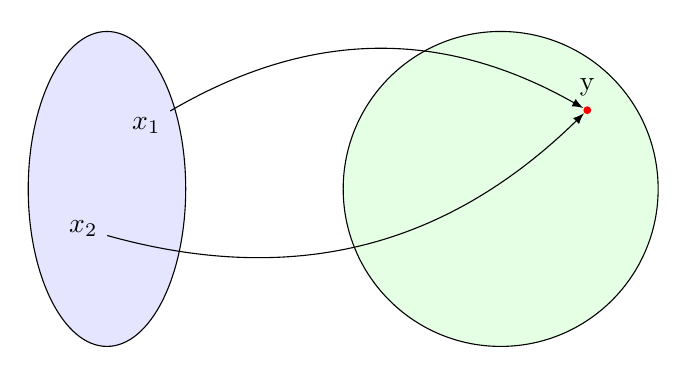
\begin{tikzpicture}
      \draw[fill=blue!10] (0,0) ellipse (1 and 2);
      \draw[fill=green!10] (5,0) ellipse (2 and 2);
      \node[fill,color=red,circle,inner sep=1pt,label=y](point) at (6.1,1) {};
      \node(x1) at (.5,.8) {$x_1$};
      \node(x2) at (-.3,-.5) {$x_2$};
      \draw[-latex,bend left] (x1) to (point);
      \draw[-latex,bend right] (x2) to (point);
    \end{tikzpicture}
    \caption{Trapdoor one-way function $f \in F$}
  \end{figure}
\end{frame}

\subsection{Superposition Stage}
\begin{frame}[label=current]{Construction of QFactory}
  Initial state :\\
  \cqubit{00}\cotimes\cqubit{00}\cotimes\cqubit{00}%
  \cotimes\cqubit{00}\cotimes\cqubit{00}\cotimes\cqubit{00}\\
\end{frame}
\begin{frame}[label=current]{Construction of QFactory}
  \begin{columns}[onlytextwidth]
    \begin{column}{.7\textwidth}
      Superposition :\\
      \hspace{.04\textwidth}\cqubit{00}\cotimes\cqubit{00}\cotimes\cqubit{00}%
      \cotimes\cqubit{00}\cotimes\cqubit{00}\cotimes\cqubit{00}\\
      + \cqubit{00}\cotimes\cqubit{00}\cotimes\cqubit{11}%
      \cotimes\cqubit{00}\cotimes\cqubit{00}\cotimes\cqubit{00}\\
      + \cqubit{00}\cotimes\cqubit{11}\cotimes\cqubit{00}%
      \cotimes\cqubit{00}\cotimes\cqubit{00}\cotimes\cqubit{00}\\
      + \cqubit{00}\cotimes\cqubit{11}\cotimes\cqubit{11}%
      \cotimes\cqubit{00}\cotimes\cqubit{00}\cotimes\cqubit{00}\\
      + \dots \strut\\
      + \cqubit{11}\cotimes\cqubit{11}\cotimes\cqubit{11}%
      \cotimes\cqubit{00}\cotimes\cqubit{00}\cotimes\cqubit{00}\\
    \end{column}
    \begin{column}{.3\textwidth}
      \only<2>{
        \begin{align*}
          \ket{\phi}
          &= \ket{0}\otimes\ket{000}\\
          &~ + \ket{1}\otimes\ket{000}\\
          &~ + \ket{2}\otimes\ket{000}\\
          &~ + \ket{3}\otimes\ket{000}\\
          &~ + \ket{4}\otimes\ket{000}\\
          &~ + \ket{5}\otimes\ket{000}\\
          &~ + \ket{6}\otimes\ket{000}\\
          &~ + \ket{7}\otimes\ket{000}\\
          &= \sum_{i=0}^{2^n-1} \ket{i}\otimes\ket{0}
        \end{align*}
      }
    \end{column}
  \end{columns}
\end{frame}
\abovedisplayskip=7pt
\abovedisplayshortskip=7pt
\belowdisplayskip=7pt
\belowdisplayshortskip=7pt

\subsection{Application of $f$ Stage}
\begin{frame}[label=current]{Application of $f$ Stage}
  \begin{columns}
    \begin{column}{.4\textwidth}
      \begin{block}{Projection}
        Server applies the following unitary $U_f$:
        \begin{align*}
        & \ket{x}\otimes\ket{0} \xrightarrow{U_f} \ket{x}\otimes\ket{f(x)}
        \end{align*}
        Applying $U_f$ on the previous superposition, results in:
        \begin{align*}
          & \sum_{i=0}^{2^n-1} \ket{i}\otimes\ket{0}\\
          \xrightarrow{U_f} & \sum_{i=0}^{2^n-1} \ket{i}\otimes\ket{f(i)}
        \end{align*}
        Then, the server measures the second register (in the computational basis), obtaining the measurement result a classical string $y \in Imf$, and the resulting state after the measurement is: 
        \begin{align*}
          (\ket{x_1} + \ket{x_2})\otimes\ket{y}
        \end{align*}
        % \vspace{-1cm}\\
        then he sends $y$ to the client.
      \end{block}
    \end{column}
    \vrule{}
    \quad
   
    \begin{column}{.5\textwidth}
    
      Example:
      \begin{align*}
        \ket{\phi'}
        &= \xxcancel<2>{\ket{0}\otimes\textcolor{red}{\ket{4}}}\\
        &~+ \ket{1}\otimes\textcolor{blue}{\ket{2}}\\
        &~+ \xxcancel<2>{\ket{2}\otimes\textcolor{green}{\ket{6}}}\\
        &~+ \xxcancel<2>{\ket{3}\otimes\textcolor{red}{\ket{4}}}\\
        &~+ \xxcancel<2>{\ket{4}\otimes\textcolor{orange}{\ket{8}}}\\
        &~+ \xxcancel<2>{\ket{5}\otimes\textcolor{green}{\ket{6}}}\\
        &~+ \xxcancel<2>{\ket{6}\otimes\textcolor{orange}{\ket{8}}}\\
        &~+ \ket{7}\otimes\textcolor{blue}{\ket{2}}
      \end{align*}
      \uncover<2>{Mesure un 2: $(\ket{1} + \ket{7})\otimes\textcolor{blue}{\ket{2}}$}
    \end{column}
   
  \end{columns}
\end{frame}

\subsection{Squeezing Stage}
\begin{frame}[label=current]{Construction}
  \Wider{
    \begin{block}{Squeezing Stage}
      
      Tranformation: $n$ qubit state $\ket{x_1} + \ket{x_2}$ $\rightarrow$ 1 qubit state $\ket{+_\theta}$\\
      Algorithm:
      \begin{itemize}
      \item Client chooses at random $\alpha_i \in \{0,1\}^3$ and sends $\alpha_i$ to the Server for $i \in \{1, 2, ..., n-1\}$ ;
      \item Server measures each on the first $n - 1$ qubits of the state $\ket{x_1} + \ket{x_2}$ in the basis $\{\ket{+_{\alpha_i\frac{\pi}{4}}}, \ket{-_{\alpha_i \frac{\pi}{4}}}\}$, obtaining measurement results $b_i$, which he sends back to the Client;
      \end{itemize}
      Result: The last (unmeasured) qubit is in the state $\ket{+_\theta}$, where:
      \begin{equation*}
        \theta = \frac{\pi}{4}(-1)^{x_{1,n}} \sum_{i = 1}^{n - 1} (x_{1,i} - x_{2,i})(4b_i + \alpha_i) \bmod 8
      \end{equation*}
      Client (using the secret $s$) can efficiently compute $\theta$, while $\theta$ looks completely random to the Server. 
    \end{block}
  }
\end{frame}


\subsection{Conclusions}
\begin{frame}{Summary of Results}
    \begin{figure}[ht]
    \centering
    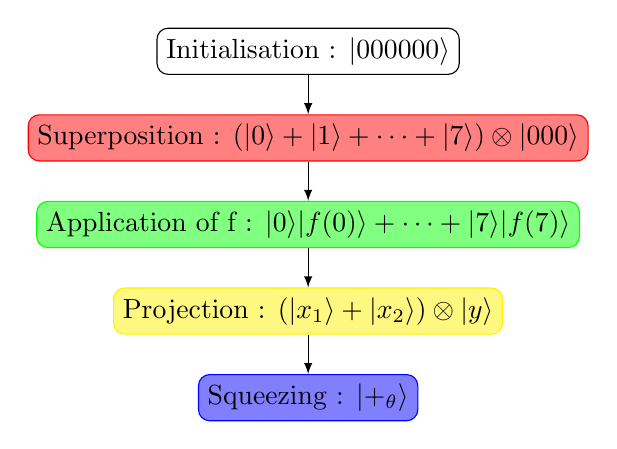
\begin{tikzpicture}[scale=0.5,node distance=.5, every node/.style={rounded corners}]
      \node[draw=black,fill=white,](init){Initialisation : $\ket{000000}$};
      \node[draw=red,fill=red!50,below= of init](superposition){Superposition : $(\ket{0}+\ket{1}+\dots+\ket{7}) \otimes \ket{000}$};
      \node[draw=green,fill=green!50,below= of superposition](appf){Application of f : $\ket{0}\ket{f(0)}+\dots+\ket{7}\ket{f(7)}$};
      \node[draw=yellow,fill=yellow!50,below= of appf](projection){Projection : $(\ket{x_1} + \ket{x_2}) \otimes \ket{y}$};
      \node[draw=blue,fill=blue!50,below= of projection](squeezing){Squeezing : $\ket{+_\theta}$};
      % Flèches
      \draw[-latex] (init) to (superposition);
      \draw[-latex] (superposition) to (appf);
      \draw[-latex] (appf) to (projection);
      \draw[-latex] (projection) to (squeezing);
    \end{tikzpicture}
    \caption{Summary of Construction}
  \end{figure}
\end{frame}

\begin{frame}[label=current]{Circuit of QFactory}
  \begin{tikzpicture}[remember picture,overlay]
    \draw[fill=red!40] ($(current page.south west)+(1.2,6.8)$)
    rectangle  ($(current page.south west)+(1.65,2.8)$);
    \draw[draw=green!40, fill=green!40] ($(current page.south west)+(1.86,0.71)$)
    rectangle  ($(current page.south west)+(3.42,6.67)$);
    \draw[fill=yellow!40] ($(current page.south west)+(3.61,0.61)$)
    rectangle  ($(current page.south west)+(4.18,2.39)$);
    \draw[fill=blue!40] ($(current page.south west)+(4.22,2.71)$)
    rectangle  ($(current page.south west)+(12.18,6.98)$);
  \end{tikzpicture}
  \resizebox{\textwidth}{!}{%
    \Qcircuit @C=1em @R=2em {
      \lstick{\ket{0}} & \gate{H} & \multigate{7}{\qquad U_{f_s}\qquad} & \qw    & \ctrl{1} & \gate{R(-\alpha_1)} & \gate{H}            & \meter   &          &                                  &          &       \\
      \lstick{\ket{0}} & \gate{H} & \ghost{\qquad U_{f_s} \qquad}       & \qw    & \gate{Z} & \ctrl{1}            & \gate{R(-\alpha_2)} & \gate{H} & \meter   &                                  &          &       \\
      \lstick{\ket{0}} & \gate{H} & \ghost{\qquad U_{f_s} \qquad}       & \qw    & \qw      & \gate{Z}            &                     &          &          &                                  &          &       \\
      \lstick{\vdots}  & \vdots   &                                     & \vdots &          &                     & \vdots              &          & \ctrl{1} & \gate{R(-\alpha_{n-1})}          & \gate{H} & \meter \\
      \lstick{\ket{0}} & \gate{H} & \ghost{\qquad U_{f_s} \qquad}       & \qw    & \qw      & \qw                 & \dots               &          & \gate{Z} & \measuretab{\mbox{Output qubit}} &          &       \\
      \lstick{\ket{0}} & \qw      & \ghost{\qquad U_{f_s} \qquad}       & \meter &          &                     &                     &          &          &                                  &          &       \\
      \lstick{\vdots}  & \vdots   &                                     & \vdots &          &                     &                     &          &          &                                  &          &       \\ 
      \lstick{\ket{0}} & \qw      & \ghost{\qquad U_{f_s} \qquad}       & \meter &          &                     &                     &          &          &                                  &          &       \\
    }
  }
\end{frame}

\begin{frame}{Conclusions and Future Work}
  
\end{frame}

\begin{frame}{Questions}
  \begin{figure}[ht]
    \centering
    
\includegraphics[width=\textwidth,height=0.8\textheight,keepaspectratio]{figures/merci.jpg}
  \end{figure}
\end{frame}

\end{document}

%%% Local Variables:
%%% mode: latex
%%% TeX-master: t
%%% End:
